\chapter{Die Basics}
\pagestyle{empty}

Im Ersten Kapitel werden wir die Grundlagen der Programmierung lernen.

Wir werden rausfinden, was ein Compiler ist, wie ein Programm abläuft und wie
man es startet. Wir werden Benutzereingaben verarbeiten und Ausgaben an die
Nutzerin geben. Wir lassen den Computer Rechnungen für uns anstellen und
lernen, was der Kontrollfluß ist -- und wie man ihn beeinflusst. Zuletzt werden
wir Vektoren kennenlernen und unser erstes nützliches Progamm schreiben.

\pagestyle{fancy}
\setcounter{chapter}{-1}
\chapter{Vorbereitung eigener Computer}
\pagestyle{empty}
Dieses Kapitel dient der Vorbereitung privater Computer, um daran den Kurs  zu bearbeiten. 
Wir werden in diesem Fall den proprietären Editor „Visual Studio Code“ verwenden, welcher \href{https://code.visualstudio.com/Download}{hier} heruntergeladen werden kann.\\

\pagestyle{fancy}
\textbf{Linux}

\pagestyle{empty}

Falls ihr privat bereits ein Linux-System nutzt.
\begin{enumerate}
	\item Optional: Alternativ zu Visual Studio Code, könnt ihr auch eine Quelloffene Version des Editors verwenden.
		Da die Installation dieser Version je nach Distribution variiert, verweisen wir euch an dieser Stelle an eine kurze Internetrecherche.
	\item Installiert mit eurem Packagemanager \texttt{g++} und ggf. \texttt{unzip}, sowie \texttt{wget}.
	\item Das Archiv mit den Vorkursdateien könnt ihr mit \\
		\texttt{wget https://mathphys.info/vorkurs/pvk/vorkurs.zip} herunterladen.
	\item Mit \texttt{unzip vorkurs.zip} könnt ihr dieses entpacken.
\end{enumerate}
\textbf{Windows}

\pagestyle{empty}
Um dem Kurs unter Windows folgen zu können sollte zunächst eine Linux-Umgebung erzeugt werden, in der die entsprechenden Tools zur Verfügung stehen. Dafür muss zunächst das so genannte Windows-Subsystem für Linux (kurz WSL) aktiviert werden.
Wie der Name bereits vermuten lässt, erlaubt es das WSL, eine Linux-Umgebung unter Windows zu nutzen.
In dieser werden wir dann die nötigen Tools installieren.
\begin{enumerate}
	\item Zunächst muss mittels PowerShell das WSL aktiviert werden. Dafür kann man im Suchfeld des Windows-Desktops einfach nach „PowerShell“ suchen.
	Durch einen Rechtsklick kann diese als Administrator gestartet werden, was für die Aktivierung notwendig ist.
	\item Hat man die PowerShell als Administrator geöffnet, kann das WSL durch den Befehl \texttt{wsl -{}-install} aktivieren.
	\item Das System startet danach einen Download, diesen durchlaufen lassen, und anschließend den PC neu starten.
	\item Nach dem Neustart kann in den Programmen „Ubuntu“ gestartet werden. 
		Wenn ihr an dieser Stelle „Ubuntu“ nicht auswählen könnt, dann ist die Installation unter Umständen noch nicht fertig.
		Startet in diesem Fall die PowerShell erneut als Administrator und führt erneut \texttt{wsl -{}-install} aus.
	\item In dem erscheinenden Terminal wird zunächst um die Erstellung eines neuen Nutzers für die Linux-Umgebung gebeten. 
		Hierbei könnt ihr Nutzername und Passwort frei wählen. Bitte notiert euch diese, da ihr sie noch braucht.\\
		\textbf{Hinweis zum setzen des Passworts:} Anders als bei Windows werden hier bei der Eingabe keine Sternchen, oder ähnliche Symbole erscheinen, die als Platzhalter für bereits eingegebene Symbole erscheinen. 
		Das Passwort muss also „blind“ eingegeben werden. Um hier ein eventuelles Vertippen auszuschließen, muss das Passwort nach der ersten Eingabe erneut bestätigt werden.
	\item Bevor ihr neue Tools installiert, solltet ihr euer System updaten. Gebt dazu ins Terminal folgende Befehle ein: \texttt{sudo apt update} und danach \texttt{sudo apt upgrade}. Im Allgemeinen empfiehlt es sich, diese Befehle im regelmäßigen Abstand auszuführen um euer System aktuell zu halten. Ihr werdet hier eventuell nach einem Passwort gefragt, ihr müsst hier das eben von euch gesetzte verwenden.
	\item Im Anschluss müssen im Terminal mittels \texttt{sudo apt install gdb g++ unzip -y} die nötigen Tools installiert werden. 
		Der Start des Vorgangs muss dabei wieder mit dem vorhin gesetzten Passwort bestätigt werden. 
		(Auch hier werden keine Sternchen oder Ähnliches für bereits eingegeben Symbole angezeigt)
	\item Jetzt könnt ihr die Dateien des Kurses mittels \\
		\texttt{wget https://mathphys.info/vorkurs/pvk/vorkurs.zip} herunterladen.
	\item Abschließend könnt ihr das Archiv mit \texttt{unzip vorkurs.zip} entpacken.
	\item Die Dateien des Vorkurses können nun mittels \texttt{code vorkurs} über das Terminal geöffnet werden.
\end{enumerate}

\textbf{MacOS}

\pagestyle{empty}

Das Setup unter MacOS ist im Vergleich zu Windows recht einfach.

\begin{enumerate}
	\item Öffnet ein Terminal.
	\item Tippt \texttt{g++} ein.
	\item Bestätigt in dem erscheinenden Fenster die Installation.
	\item Die Dateien des Vorkurses können \href{https://mathphys.info/vorkurs/pvk/vorkurs.zip}{hier} heruntergeladen werden.
	\item Entpackt die Dateien in ein Verzeichnis eurer Wahl.
	\item In Visual Studio Code könnt ihr dann über den Explorer auf die Dateien des Kurses zugreifen.
\end{enumerate}

\lesson{Die Shell}

Wenn ihr bisher nur mit Windows oder Mac gearbeitet habt, habt ihr
wahrscheinlich in der letzten Lektion nebenbei etwas neues Kennen gelernt: Die
Shell.

Auch wenn sich unter Linux zunehmend Desktopumgebungen, wie man sie von
kommerziellen Betriebssystemen kennt verbreiten, bleibt die Shell immer noch das
Mittel der Wahl, wenn man sich mit dem System auseinander setzen, oder auch
allgemein arbeiten will. Wir erachten zumindest die Shell als wichtig genug, um
euch direkt zu Beginn damit zu konfrontieren.

Wann immer ihr über die Anwendungen ein Terminal startet, wird dort drin
automatisch auch eine Shell gestartet. Die beiden Konzepte sind tatsächlich so
eng miteinander verknüpft, dass ihr euch um die Unterschiede erst einmal keine
Gedanken machen müsst - wann immer ihr Shell oder Terminal hört, denkt einfach
an das schwarze Fenster mit dem Text. Das ist auch das wesentliche Merkmal der
Shell, sie ist ein Textbasiertes interface zu eurem Computer. Ihr gebt Befehle
ein, sie gibt euch Text zurück und auf diese Weise könnt ihr eigentlich alles
machen, was ihr sonst gewohnterweise mit der Maus und grafischen Oberflächen
tun würdet.

Wenn die Shell auf eure Befehle wartet, zeigt sie euch den so genannten
\emph{Prompt} an. Er enthält unter anderem euren Nutzernamen und das aktuelle
Verzeichnis ($\sim$ steht dabei für euer Nutzerverzeichnis, ein spezieller
Ordner, der eurem Account zugeordnet ist und in dem ihr alle Rechte besitzt,
dieser wird auch \emph{home} genannt).

Wenn ihr in ein anderes Verzeichnis wechseln wollt, könnt ihr das (wie ihr
bereits in der ersten Lektion gelernt habt) mit dem Befehl \texttt{cd} tun,
gefolgt von dem Namen des Verzeichnis. Um zurück zu gehen, könnt ihr das
spezielle Verzeichnis \texttt{..} (also zwei Punkte) angeben, welches für das
nächst höher liegende Verzeichnis steht. Wenn ihr euch den Inhalt des
Verzeichnisses anschauen wollt, könnt ihr dafür den Befehl \texttt{ls}
benutzen. Um herauszufinden, in welchem Verzeichnis ihr euch befindet, könnt
ihr \texttt{pwd} nutzen, zum Kompilieren von \Cpp-Programmen habt ihr den Befehl
\texttt{g++} kennengelernt. Solltet ihr Hilfe zu irgendeinem Befehl benötigen,
könnt ihr den Befehl \texttt{man} (für „Manual“) geben, gefolgt von dem Befehl,
zu dem ihr Hilfe braucht (über \texttt{man} werden wir später noch
ausführlicher reden).

\newpage

\begin{praxis}
    \begin{enumerate}
        \item Öffnet ein Terminal und gebt die folgenden Befehle ein:
              \inputshell{basics.sh}
    \end{enumerate}
\end{praxis}

\begin{spiel}
    \begin{enumerate}
        \item Versucht selbst durch euer Nutzerverzeichnis (\emph{home}) zu navigieren.
              Wie viele Lektionen hat der Vorkurs in diesem Verzeichnis?
        \item Was passiert, wenn ihr euer Homeverzeichnis verlasst (\texttt{cd ..}
              während ihr darin seid)?
        \item Versucht in der manpage von ls (\texttt{man ls}) zu stöbern und die
              verschiedenen Parameter, mit denen ihr das Verhalten steuern könnt zu
              erforschen. Findet ihr heraus, wie ihr den Verzeichnisinhalt in einem
              langen Listenformat (long listing format) anzeigen lassen könnt (in dem
              unter anderem auch die Dateigröße zu jeder Datei steht). 
              Hinweis: mit \texttt{\textbackslash Suchbegriff} kann innerhalb von \texttt{man} gesucht werden.
        \item Um schnell mit der Shell zu arbeiten gibt es einige Tricks. 
        Damit lange Dateinamen nicht immer komplett eingegeben werden müssen, gibt es die sogenannte \texttt{tab completion}. 
        Um bereits eingegebene Befehle nochmals auszuführen die \texttt{history}. Finde heraus wie diese funktionieren!
    \end{enumerate}
  \end{spiel}


Falls euch das alles verwirrt, fragt entweder direkt nach oder wartet auf
Lektion 6, da geht es zu Manpages noch mal ins Detail.

Ihr findet unter \url{http://blog.ezelo.de/basic-linux-befehle/} auch noch mal
die wichtigsten Befehle zusammengefasst.

\textbf{Quiz 2}\\
\textit{Was passiert, wenn ihr \texttt{cd .} ausführt?}
\begin{enumerate}[label=\alph*)]
    \item Ihr geht in ein zufälliges Unterverzeichnis
    \item Ihr bleibt im gleichen Verzeichnis
    \item Ihr verlasst euer aktuelles Verzeichnis
    \item Ihr geht direkt in euer Homeverzeichnis
\end{enumerate}
\lesson{Hello world}

Die erste Lektion beschäftigt sich alleine mit der Frage, was eigentlich eine
Programmiersprache überhaupt ist und wie wir den Computer dazu bringen können,
daraus etwas zu machen, was er ausführen kann.
Traditionell wird hierfür ein Programm herangezogen, das „Hallo Welt!“ ausgibt. \\


\textbf{Wie entsteht ein Programm?}

Wie bringen wir also den Computer dazu, diese Ausgabe zu generieren? - intern besteht er aus
vielen Transistoren (wenn ihr nicht wisst, was das ist, denkt an winzige
Schalter - näheres folgt im späteren Studium), die nur die Zustände „an“ und „aus“ kennen.
Wir müssen also die Anweisung „gebe Hallo Welt aus“ in ein Format übersetzen, was nur „an“ und
„aus“ bzw. „0“ und „1“ benutzt.

Nun ist es umständlich, ein umfangreiches Programm in 0en und 1en zu schreiben. Deswegen benutzt man
heutzutage so genannte Hochsprachen, um Programme zu beschreiben. Wir
beschreiben also den Programmablauf in einer von Menschen lesbaren und
(leicht) verstehbaren Sprache, welche später in 0en und 1en übersetzt wird und anschließend vom Computer lesbar ist und ausgeführt werden kann.
Wir benutzen die Hochsprache \Cpp. Die Programmbeschreibung in
\Cpp legen wir dabei in einer einfachen Textdatei ab. Damit wir auf anhieb erkennen, um welche Hochsprache es sich handelt, hat es sich etabliert die Endung
\texttt{.cpp} an den Dateinamen anzuhängen.

Die Übersetzung aus der von Menschen lesbarer Hochsprache in Maschinensprache erledigt für uns der \emph{Compiler}.
Der Compiler generiert aus der Textdatei also Maschinencode generiert. Der Compiler für \Cpp, den wir in diesem Kurs
benutzen wollen, heißt \texttt{g++}.

Vereinfacht sieht der Prozess zur Programmerstellung also wie folgt aus:


\begin{tikzpicture}
    \node (1) at (0,0) [rectangle, draw] {Programmcode schreiben (Hochsprache)};
    \node (2) at (6,0) [rectangle, draw] {Kompilieren};
    \node (3) at (9,0) [rectangle, draw] {Ausführen};
    \draw[->, blue!50, very thick] (1) to (2);
    \draw[->, blue!50, very thick] (2) to (3);
\end{tikzpicture} \\

\textbf{Wie gehe ich dabei vor?}

Um den Programmcode in eine Textdatei zu schreiben verwenden wir einen Texteditor.
Dies kann mit fast jedem einfachen Texteditor bewerkstelligt werden. Populäre konsolenbasierte Editoren sind \texttt{vim} und \texttt{nano}. Es existieren aber auch grafische Editoren, die speziell für das Schreiben von Programmcode entwickelt wurden, wie \texttt{Visual Studio Code} oder \texttt{CLion}\footnote{https://www.jetbrains.com/community/education}.
Um dem Compiler zusagen, welche Textdatei er in ein Programm übersetzen soll, verwenden wir die sogenannte Shell. Vorerst reicht uns zu wissen, dass die Shell
ein Werkzeug ist, um dem Computer spezifisch zu sagen, was er machen soll (mehr dazu im folgenden Kapitel). In Ubuntu verwenden wir hierzu das Terminal, ebenso in MacOS,
unter Windows CMD oder Powershell. Ein Befehl für \texttt{g++} (dem Compiler für \Cpp) sieht beispielsweise wie folgt aus:

\begin{center}
    \texttt{g++ -o outputDatei zuKompilierendeDatei.cpp}
\end{center}
Hierbei legen wir mit dem Parameter \texttt{-o} (o für output) und dem ersten darauf folgenden Argument den Namen der Ausgabedatei fest.

Nachdem \texttt{g++} uns also ein Maschinencodefile -- die \texttt{outputDatei} --
erzeugt hat, können wir es zur Ausführung bringen. Dies kann im Terminal mit einem Punkt und einem Slash vor dem Dateinamen geschehen. Also:
\begin{center}
    \texttt{./outputDatei}
\end{center}



\begin{praxis}

    \textbf{Erstes Programm in \Cpp schreiben}

    \begin{enumerate}
        \item Erstelle eine neue, leere Datei in einem Editor deiner Wahl.
        
        \item Kopiere folgenden Programmcode in den Texteditor und speichere ihn in einer Datei mit dem Namen „helloworld.cpp“ ab. 
        Das nähere Verständnis des Programmcodes ist an dieser Stelle nicht notwendig. 
    \end{enumerate}    

    \inputcpp{helloworld.cpp}

    \textbf{\Cpp-Code komplieren und Programm erstellen }
  
    \begin{enumerate}
        \item Öffne ein Terminal (Konsole), ihr findet das Terminal unter Ubuntu oben links unter „Applications“ als „Terminal“ oder mittig unten als das zweite Symbol von links.
        \item Wechselt mit dem Befehl \texttt{cd [PFAD]} in das Verzeichnis (Ordner), indem ihr eure Textdatei erstellt habt (\texttt{[PFAD]} muss hierbei durch den Speicherort der Datei ersetzt werden).
              Was dieser Befehl genau tut und wie er funktioniert, erfahrt ihr in Lektion 2.
        \item In diesem Verzeichnis liegt nun eine Datei mit dem Namen \texttt{helloworld.cpp}.
              Benutzt \texttt{g++}, um diese zu einer Datei (in diesem Fall dem Programm) \texttt{hello} zu
              kompilieren. Orientiert euch dazu an den folgenden Befehlen. (siehe Diagramm)
        \item Führt die Datei \texttt{hello} aus.
    \end{enumerate}
\end{praxis}


Zur besseren Übersichtlichkeit hier der ganze Vorgang noch mal in einem
Diagramm:

% TODO: Buttugly, but well... - its gonna stay this way
\begin{center}
    \resizebox{\textwidth}{!}{
        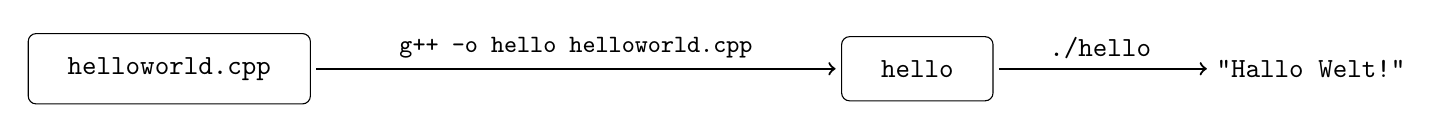
\begin{tikzpicture}
            \node (nHelloWorldCpp) [ shape=rectangle, rounded corners = 0.1cm, draw=black, inner xsep=0.5cm, inner ysep = 0.3cm ] {\texttt{helloworld.cpp}};
            \node (nHello) [ right of = nHelloWorldCpp, node distance = 9.5cm, shape=rectangle, rounded corners = 0.1cm, draw = black, inner xsep = 0.5cm, inner ysep = 0.3cm ] {\texttt{hello}};
            \draw [->, thick, shorten >= 2pt, shorten <= 2pt ] (nHelloWorldCpp) -- (nHello) node [ midway, above, font = \small ] { \texttt{g++ -o hello helloworld.cpp}} ;
            \node (nOutput) [ right of = nHello, node distance = 5cm, shape=rectangle ] {\texttt{"Hallo Welt!"}};
            \draw [->, thick, shorten <= 2pt] (nHello) -- (nOutput) node [ midway, above ] {\texttt{./hello}};
        \end{tikzpicture}
    }
\end{center}

\newpage

\begin{spiel}

Ihr könnt nun versuchen, den Quellcode selbst zu verändern und damit ein wenig
herumzuspielen. Öffnet dazu einen Editor und öffnet die Datei
\texttt{vorkurs/lektion01/helloworld.cpp}\footnote{am besten öffnet ihr in VSCode den gesamten Vorkurs-Ordner}. Denkt daran, nach jeder Änderung die Datei zu speichern und
im Terminal neu zu kompilieren und auszuführen.

Dinge, die ihr ausprobieren könntet sind zum Beispiel:
\begin{enumerate}
    \item Was passiert, wenn ihr „Hello world!“ in etwas anderes ändert?
    \item Was passiert, wenn ihr die erste Zeile löscht (der Originalquellcode
        ist in diesem pdf enthalten, ihr könnt sie also später wieder
        herstellen)?
    \item Was passiert, wenn ihr das „\verb|<< std::endl|“ löscht?
    \item Wie könnte man mehrere Sätze ausgeben? Wie könnte man mehrere Zeilen
        ausgeben?
\end{enumerate}
\end{spiel}

\textbf{Quiz 1}\\
\textit{Was passiert, wenn ihr \texttt{Hello world} durch etwas anderes ersetzt?}
\begin{enumerate}[label=\alph*)]
    \item Das andere wird ausgegeben
    \item Es gibt einen Fehler
    \item Das Programm tut garnichts mehr
    \item Das Programm gibt trotzdem \texttt{Hello world} aus
\end{enumerate}

\lesson{Input und Output}

Nachdem wir ein bisschen Vertrauen in die shell entwickelt haben und zumindest
bereits unser erstes Programm kompiliert, wollen wir nun etwas spannendere
Dinge tun. Nach wie vor müsst ihr nicht jede Zeile eures Programmes verstehen.
Sollte euch bei einer bestimmten Zeile trotzdem interessieren, was genau sie
tut, versucht doch eventuell sie zu entfernen, das Programm zu kompilieren und
schaut, was sich ändert.

Wir wollen uns nun mit grundlegendem input und output vertraut machen, denn
erst wenn euer Programm mit einer Benutzerin interagiert, wird es wirklich
nützlich. Wir haben in der ersten Lektion bereits \texttt{cout} (für
\emph{console out}) kennengelernt, um Dinge auszugeben. Nun nutzen wir
\texttt{cin}, um Eingaben des Benutzers entgegen zu nehmen. Jedes Programm
unter Linux (und übrigens auch Mac OS oder Windows) kann auf diese Weise
Eingaben von der Nutzerin entgegen nehmen und Ausgaben liefern. Das ist auch
der Grund, warum die Konsole so wichtig ist und es viele Dinge gibt, die nur
mittels einer Konsole gelöst werden können: Während es viele Stunden dauert,
ein grafisches Interface zu programmieren, über die man mit dem Programm mit
der Maus kommunizieren kann, kann praktisch jeder ein textbasiertes
Konsoleninterface schreiben. Linux ist ein Ökosystem mit einer gewaltigen
Anzahl tools für jeden denkbaren Zweck und bei den meisten haben die Autorinnen
sich nicht die Mühe gemacht, extra eine grafische Oberfläche zu entwickeln.

Nun aber direkt zur Praxis:

\begin{praxis}
    \begin{enumerate}
        \item Öffnet die Datei \texttt{vorkurs/lektion03/helloyou.cpp} in eurem Texteditor
        \item Öffnet ein Terminal und wechselt in das Verzeichnis \texttt{vorkurs/lektion03}
        \item Kompiliert im Terminal die Datei (\texttt{g++ -o helloyou
                  helloyou.cpp}) und führt sie aus (\texttt{./helloyou})
        \item Versucht verschiedene Eingaben an das Programm und beobachtet, was passiert
    \end{enumerate}

    \inputcpp{helloyou.cpp}
\end{praxis}

\begin{spiel}
\begin{enumerate}
    \item Versucht, zu verstehen, was die einzelnen Teile des Programms tun. An
        welcher Stelle erfolgt die Eingabe? Was passiert dann damit?
    \item Erweitert das Programm um eigene Fragen und Ausgaben. Vergesst nicht,
        dass ihr das Programm nach jeder Änderung neu kompilieren und testen
        müsst.
\end{enumerate}
\end{spiel}

\textbf{Quiz 3}\\
\textit{Was passiert, wenn \texttt{std::cin >> eingabe;} vor \texttt{std::string eingabe;} steht?}
\begin{enumerate}[label=\alph*)]
    \item Das Programm funktioniert ganz normal
    \item Es wird \texttt{eingabe} ausgegeben
    \item Es wird \texttt{Hello} ausgegeben
    \item Das Programm kann nicht kompiliert werden
\end{enumerate}

\lesson{Preprocessing, Compiler, Assembler, Linker}

In der letzten Lektion habt ihr bereits das erste mal ein Programm kompiliert,
d.h. ihr habt eine für Menschen lesbare Datei in eine für Computer lesbare Datei 
übersetzt. Jetzt wollen wir uns etwas genauer anschauen was dabei eigentlich passiert. 
Ihr müsst dabei jetzt nicht jedes Detail vestehen, aber es ist praktisch zu
wissen, wie der Compile Vorgang funktioniert um manche Fehlermeldungen zu verstehen.

In Lektion 1 haben wir vereinfacht dargestellt, dass der Compiler eine
Quelltextdatei mit der Endung \texttt{.cpp} nimmt und daraus direkt eine
ausführbare Datei erstellt. Die Schritte, die hier eigentlich in einem Befehl
durchgeführt werden, aber zu trennen sind, sind das \emph{Preprocessing}, das \emph{Kompilieren}, das
\emph{Assemblieren} und das \emph{Linken}.

Beim Preprocessing werden alle \texttt{\#include}-Anweisungen aufgelöst.
Das ist der erste Schritt, der passiert, wenn wir \texttt{g++} 
aufrufen. Das Ergebnis des Preprocessings ist ein erweitertes\Cpp-Programm, das nur noch die
\Cpp-Features enthält, die wir auch wirklich benutzen. Das ist der Grund, warum wir
in den bisherigen Lektionen immer \texttt{g++ -o helloworld helloworld.cpp} benutzt haben,
obwohl wir in \texttt{helloworld.cpp} auch \texttt{\#include <iostream>} stehen haben
-- der Compiler hat das schon für uns erledigt.

Das Kompilieren übersetzt unseren erweiterten \Cpp-Code in eine Zwischenform, so genannten
\emph{Assembler}. In Lektion 1 haben wir den Maschinencode angesprochen, in der
Befehle und Parameter an Befehle in 1en und 0en dargestellt werden. Assembler
ist quasi die nächst höhere Evolutionsstufe -- statt die Befehle binär zu
kodieren, gibt es für jeden Befehl ein so genanten \emph{mnemonic}, also ein
merkbares kurzes Wort. Ein Befehl ist allerdings deutlich weniger mächtig, als
z.B. eine Anweisung in \Cpp. Früher wurden ganze Betriebssysteme in Assembler
geschrieben, da es einfach nichts Besseres gab, heutzutage ist Assembler bis
auf die exotischsten Anwendungsfelder eigentlich ausgestorben, da es viel zu
anstrengend und Fehleranfällig ist. Der Compiler tut aber noch mehr, als
einfach nur in diese Zwischensprache zu übersetzen -- er führt auch
\emph{Optimierungen} durch, d.h. er sortiert Anweisungen um, damit der Code
schneller läuft, aber das Gleiche tut. Dieser Prozess ist sehr umständlich,
aber heutige Compiler sind tatsächlich so gut im Optimieren, dass sie meistens
deutlich schnelleren Code erzeugen, als ein Mensch es je könnte.

Der nächste Schritt ist dann das Assemblieren. Das übersetzt den Assembler des
ersten Schrittes tatsächlich in Maschinensprache (genauer: In ein Dateiformat,
welches ELF heißt, welches dann die Maschinensprache plus einiger
Meta-Informationen enthält). Der Assembler erzeugt so genannte
\emph{Objectfiles}, die meistens die Endung \texttt{.o} haben (und im
ELF-Format sind). Ein Objectfile enthält dann mehrere Funktionen (in
Maschinencode) und Variablen, die es \emph{exportieren} kann, d.h. Funktionen
anderer Objectfiles die dagegen (im nächsten Schritt) gelinkt werden, können
diese Variablen und Funktionen sehen. Der Vorteil, diesen Schritt vom
vorhergehenden zu trennen ist, dass wir wenn wir wollen auch nur kompilieren
können und den resultierenden Assembler betrachten -- das kann uns helfen,
Engpässe in unserem Code, an denen der Compiler nicht hinreichend gut optimiert
zu erkennen und möglicherweise zu verbessern. z.B. in der Spielentwicklung ist
sehr schnell laufender Code wichtig.

Der letzte Schritt ist das Linken. Hier werden mehrere Objectfiles genommen und
miteinander verbunden, zu einer ausführbaren Datei. Wenn in einer der
Objectfiles eine \texttt{main}-Funktion existiert, wird diese als
Eintrittspunkt für das Programm genommen, sonst gibt es einen
\emph{Linkerfehler}. Ein Linkerfehler tritt auch auf, wenn wir versuchen, eine
Funktion zu verwenden, die es nicht gibt (z.B. indem wir Funktionen aus einem 
Headerfile benutzen ohne das Header-File mit \texttt{#include} auch tatsächlich einzubinden).
Linkerfehler deuten also darauf hin, dass wir vergessen haben, alle
relevanten Dateien auf der Kommandozeile anzugeben, oder dass eine
\texttt{main}-Funktion fehlt, oder dass wir in mehren Dateien eine Funktion
gleichen Namens haben, oder\dots

Wenn ihr das Programm aus der letzten Lektion kompiliert passiert im Prinzip also
folgendes:

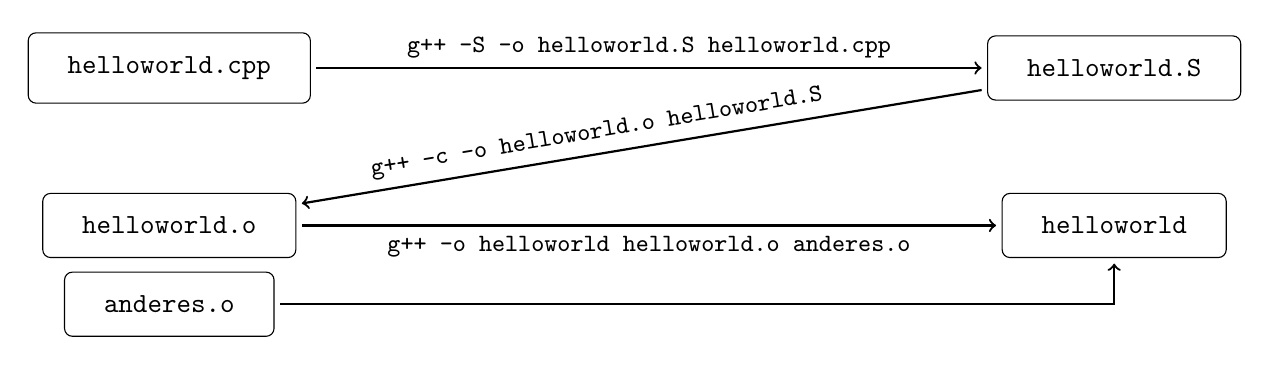
\begin{tikzpicture}
    \tikzstyle{block} = [ shape=rectangle, rounded corners = 0.1cm, draw=black, inner xsep=0.5cm, inner ysep = 0.3cm ];
    \tikzstyle{arr} = [ ->, thick, shorten >= 2pt, shorten <= 2pt ];

    \node (nHelloWorldCpp) [block] {\texttt{helloworld.cpp}};
    \node (nHelloWorldS) [block, right of = nHelloWorldCpp, node distance = 12cm] {\texttt{helloworld.S}};
    \draw [arr] (nHelloWorldCpp) -- (nHelloWorldS) node [midway,above,font=\small] {\texttt{g++ -S -o helloworld.S helloworld.cpp}};
    \node (nHelloWorldO) [block, below of = nHelloWorldCpp, node distance = 2cm] {\texttt{helloworld.o}};
    \draw [arr] (nHelloWorldS) -- (nHelloWorldO) node [pos=0.56,above,sloped,font=\small] {\texttt{g++ -c -o helloworld.o helloworld.S}};
    \node (nAnderesO) [block, below of = nHelloWorldO, node distance = 1cm] {\texttt{anderes.o}};
    \node (nHelloWorld) [block, below of = nHelloWorldS, node distance = 2cm] {\texttt{helloworld}};
    \draw [arr] (nHelloWorldO) -- (nHelloWorld) node [midway,below,font=\small] {\texttt{g++ -o helloworld helloworld.o anderes.o}};
    \draw [arr] (nAnderesO) -| (nHelloWorld) node {};
\end{tikzpicture}

Der bisherige Befehl, den wir zum Kompilieren benutzt haben, ist tatsächlich
nur ein Spezialfall von diesem: Geben wir nämlich auf der Kommandozeile eine
input-Datei an, so rät \texttt{g++} anhand der Dateierweiterung und der
Parameter, was wir damit tun wollen. Er führt dann alle Schritte, um von
unserer input-Datei zu der gewünschten zu kommen automatisch aus, wenn wir also
\texttt{g++ -o helloworld helloworld.cpp} eingeben, dann weiß der Compiler,
dass wir eine ausführbare Datei wünschen (da wir weder \texttt{-c} noch
\texttt{-S} angegeben haben) und dass er dafür preprocessen, kompilieren, assemblieren und
linken muss (da wir ihm eine \texttt{.cpp} Datei gegeben haben).
\begin{praxis}
    \begin{enumerate}
        \item \texttt{assemble.cpp} enthält ein kleines (ziemlich nutzloses)
              Programm, welches zwei Zahlen addiert und das Ergebnis ausgibt.
              Kompiliert es (nun nur der erste Schritt in dem Diagramm, nicht so, wie
              in den vergangenen Lektionen) und schaut euch das resultierende
              \texttt{.S}-file in einem Editor an. Ihr müsst nicht verstehen,
              was genau hier überall passiert, aber vielleicht findet ihr ja die
              \texttt{main}-Funktion, die Definition der Variablen und die Addition?

              Wir können nun mal Optimierung anschalten -- gebt dazu zusätzlich den
              Parameter \texttt{-O3} direkt nach dem \texttt{g++} an. Schaut euch das
              \texttt{.S}-file nun wieder im Editor an. Was fällt euch
              (im Vergleich zu vorher) auf?
        \item Assembliert eines der im vorigen Schritt erzeugten \texttt{.S} files
              in ein \texttt{.o}-File.
        \item Benennt in einem eurer bisherigen Programme die
              \texttt{main}-Funktion um und versucht, es zu kompilieren (wie in den
              bisherigen Lektionen, also alle Schritte auf einmal). Schaut euch die
              resultierenden Fehlermeldungen an. Wo wird euch der Linkerfehler
              ausgegeben?
        \item Macht die Umbenennung wieder rückgängig und kompiliert das Programm
              erneut -- übergebt aber dieses mal den Quellcode doppelt (also z.B.
              \texttt{g++ -o helloworld helloworld.cpp helloworld.cpp}). Was
              beobachtet ihr? Könnt ihr die Beobachtung erklären?
    \end{enumerate}

    \inputcpp{assemble.cpp}
\end{praxis}

\input{lektionen/variablen_datatypes}
\lesson{Arithmetik}

Wir haben in der vergangenen Lektion Variablen vom Typ \texttt{std::string}
kennengelernt. Zeichenketten zu speichern ist schon einmal ein guter Anfang,
aber wir wollen auch rechnen können, wir brauchen also mehr Typen für
Variablen.

\Cpp unterstützt eine Unmenge an Datentypen und hat auch die Möglichkeit,
eigene zu definieren. Wir wollen uns hier nur mit den wichtigsten beschäftigen.

Fangen wir mit dem wohl meist genutzten Datentyp an: Einem \texttt{int}, oder
\texttt{integer}. Dieser speichert eine ganze Zahl (mit bestimmten Grenzen, an
die wir aber erst einmal nicht stossen werden, von daher ignorieren wir sie
erst einmal frech). Mit \texttt{int}s können wir rechnen, das funktioniert in
\Cpp mit ganz normalen Rechenausdrücken, wie wir sie aus der Schule kennen,
plus den bereits angetroffenen Zuweisungen:

\inputcpp{arith1.cpp}

Wichtig ist hier, zu beachten, dass wir dem Computer ein in Reihenfolge
abgearbeitetes Programm geben, keine Reihe von Aussagen. Das bedeutet in diesem
konkreten Fall, dass wir z.B. nicht die Aussage treffen „\texttt{a} ist gleich
7“, sondern dass wir sagen „lasse zuerst \texttt{a} den Wert 7 haben. Lasse
dann \texttt{b} den Wert 19 haben. Lasse dann \texttt{c} den Wert haben, der
heraus kommt, wenn man den Wert von \texttt{b} vom Wert von \texttt{a}
abzieht“. Besonders deutlich wird dieser Unterschied bei einem Beispiel wie
diesem:

\inputcpp{arith2.cpp}

\begin{praxis}
    \begin{enumerate}
        \item Was gibt dieses Programm aus? Überlegt es euch zuerst und kompiliert
              es dann, um es auszuprobieren.
    \end{enumerate}

    Obwohl \texttt{a = a + 19} mathematisch überhaupt keinen Sinn ergibt, ist doch
    klar, was passiert, wenn man sich den Quellcode eben nicht als Reihe von
    Aussagen, sondern als Folge von \emph{Anweisungen} vorstellt. Das
    Gleichheitszeichen bedeutet dann nicht, dass beide Seiten gleich sein sollen,
    sondern dass der Wert auf der linken Seite den Wert auf der rechten Seite
    annehmen soll.

    Wie wir in diesem Beispiel ausserdem sehen, können wir nicht nur Strings
    ausgeben, sondern auch Zahlen. \texttt{std::cout} gibt sie in einer Form aus,
    in der wir etwas damit anfangen können. Genauso können wir auch über
    \texttt{std::cin} Zahlen vom Benutzer entgegen nehmen:

    \inputcpp{arith3.cpp}

    Langsam aber sicher tasten wir uns an nützliche Programme heran!

    \begin{enumerate}[resume]
        \item Schreibt ein Programm, welches von der Nutzerin zwei ganze Zahlen
              entgegen nimmt und anschließend Summe, Differenz, Produkt und Quotient
              ausspuckt.
        \item Was fällt auf, wenn ihr z.B. 19 und 7 eingebt?
        \item Findet heraus (Google ist euer Freund), wie man in \Cpp Division mit
              Rest durchführt und gebt diese zusätzlich zu den bisherigen Operationen
              mit aus\footnote{Falls ihr nicht weiterkommt, hilft euch vielleicht das
                  Stichwort „modulo“ oder „modulo-operator“ weiter.}.
        \item Was passiert, wenn ihr als zweite Zahl eine 0 eingebt?
    \end{enumerate}
\end{praxis}

\begin{spiel}
\begin{enumerate}
    \item Findet heraus, was die größte positive (und was die kleinste
        negative) Zahl ist, die ihr in einem \texttt{int} speichern könnt.
        Faulpelze nutzen Google, Lernbegierige versuchen sie experimentell zu
        ermitteln. Was passiert, wenn ihr eine größere Zahl eingebt?
    \item Wir arbeiten bisher nur mit \texttt{int}s für ganze Zahlen. Wenn wir
        mit gebrochenen Zahlen rechnen wollen brauchen wir den Datentyp
        \texttt{double}. Schreibt euer Mini Rechenprogramm so um, dass es statt
        \texttt{int}s nur noch \texttt{double} benutzt und probiert es aus.
        Achtet darauf, dass es Dezimalpunkte und Dezimalkommata gibt, wenn ihr
        überraschende Ergebnisse erhaltet.
\end{enumerate}
\end{spiel}

\textbf{Quiz 7}\\
\textit{Was passiert, wenn ihr \texttt{int} verwendet, aber eine Kommazahl eingebt?}
\begin{enumerate}[label=\alph*)]
    \item Alles hinter dem Komma wird abgeschnitten
    \item Es tritt ein Fehler auf
    \item Das Programm kompiliert nicht
    \item statt \texttt{int} wird automatisch \texttt{double} genommen
\end{enumerate}


\lesson{Der Kontrollfluss}

Wer versucht hat in der vergangenen Lektion Praxisaufgabe 5 zu lösen, wird auf der Konsole eine ähnliche Ausgabe wie folgt bekommen - einen Fehler:
\begin{minted}{text}
Gebe eine Zahl ein: 5
Gebe noch eine Zahl ein: 0
Floating point exception
\end{minted}

Das Programmcode hierfür kann beispielsweise wie folgt aussehen.

\inputcpp{arith4.cpp}

Wenn wir diesen Fehler beheben wollen, haben wir eigentlich nur zwei
Möglichkeiten: Die erste ist, die Schuld auf die Benutzerin zu schieben, warum
versucht sie auch, eine 0 einzugeben? Ich hoffe, ihr stimmt zu, dass das nicht
sehr freundlich wäre. Stellt euch vor, jedes mal, wenn ihr in einem Programm
einen Wert eingebt, auf den das Programm nicht vorbereitet ist, würde es direkt
abstürzen. Das fändet ihr vermutlich nicht so gut, es sollte doch zumindest mal
eine Fehlermeldung ausgeben und die Nutzerin informieren, dass sie was falsch
gemacht hat.

Und das ist der zweite Weg, den wir jetzt einschlagen wollen. Unser Programm
sollte am Besten, nachdem es die Eingabe von der Benutzerin entgegen genommen
hat, einfach überprüfen, ob die Division erlaubt ist oder nicht. Sollte die
Nutzerin eine 0 eingegeben haben, sollte es auf den Fehler hinweisen und sich
beenden, sonst sollte es den Quotienten ausgeben. Diese Abhängigkeit des
Verhaltens eines Programms von den Eingaben, bezeichnen wir als
\emph{Kontrollfluss}, man kann das mit einem Diagramm verdeutlichen:

\begin{center}
      \begin{tikzpicture}[auto, node distance=3cm,>=latex']
            \tikzstyle{block} = [draw, fill=blue!20, rectangle, minimum height=3em, minimum width=6em]

            \node [block] (start) {Input};
            \node [block, right of=start] (if) { $a=0$? };
            \node [block, right of=if, node distance=4cm] (fehler) { Gib Fehler aus };
            \node [block, below of=fehler,node distance =  2cm] (quotient) { Gib Quotient aus };
            \node [block, right of=fehler, node distance = 3.5cm] (ende) { Ende };

            \draw [->] (start) -- node {} (if);
            \draw [->] (if) -- node {\texttt{ja}} (fehler);
            \draw [->] (if.south) |- node [above, near end] {\texttt{nein}} (quotient);
            \draw [->] (quotient) -| node {} (ende);
            \draw [->] (fehler) -- node {} (ende);
      \end{tikzpicture}
\end{center}

Die einfachste Möglichkeit, den Kontrollfluss zu ändern, besteht in so
genannten „bedingten Anweisungen“:
\inputcpp{if.cpp}

In den Zeilen 12 bis 20 sehen wir, wie eine solche Bedingte Anweisung in \Cpp
aussieht. Wir erkennen relativ direkt unser Diagramm hier wieder: In Zeile 12
steht der „$b=0$?“ Block, in den Zeilen 13 bis 17 steht der „Gib Fehler aus“
Block und in Zeile 19 der „Gib den Quotienten aus“ Block. Die Blöcke lassen sich auch gut anhand der geschweiften Klammern und der Einrückung erkennen. Wir empfehlen euch, solche logischen Blöcke einzurücken, um die Lesbarkeit des Codes zu verbessern. Eine ausführlichere Erklärung zum coding style gibt es in Lektion \ref{sec:codingstyle}.

Beachtet allerding die doppelten Gleichheitszeichen in Zeile 12. \Cpp hat
getrennte Operatoren für Vergleiche und Zuweisungen - Doppelte
Gleichheitszeichen bedeuten Vergleich („sind diese beiden gleich?“), ein
einfaches Gleichheitszeichen bedeutet Zuweisung („mache diese beiden gleich!“).

\begin{praxis}
      \begin{enumerate}
            \item Nutzt Google, um herauszufinden, welche anderen Vergleichsoperatoren
                  es in \Cpp noch gibt. Versucht, das Programm so zu verändern, dass es
                  auf Ungleichheit testet, statt auf Gleichheit (sich sonst aber genauso
                  verhält).
            
            \item Wie würdet ihr testen, ob zwei Zahlen durch einander teilbar sind
                  (Tipp: Ihr kennt bereits die Division mit Rest in \Cpp (modulo))?
                  Schreibt ein Programm, welches zwei Zahlen von der Nutzerin entgegen
                  nimmt und ausgibt, ob die zweite Zahl die erste teilt.
      \end{enumerate}
\end{praxis}

\begin{spiel}
\begin{enumerate}
    \item Testet mit verschiedenen Eingaben, was passiert, wenn ihr in
        \texttt{if.cpp} statt zwei Gleichheitszeichen nur eines benutzt.

    \item Schreibt ein Programm, welches die Benutzerin fragt, wie sie heißt.
        Gibt sie euren eigenen Namen ein, soll das Programm begeistert über die
        Namensgleichheit sein, sonst sie einfach begrüßen.
\end{enumerate}
\end{spiel}

\textbf{Quiz 8}\\
\textit{Welche Aussagen sind korrekt?}
\begin{enumerate}[label=\alph*)]
    \item Mit \texttt{=} vergleicht man.
    \item Es darf immer nur ein \texttt{if} vor einem \texttt{else} kommen.
    \item Es darf nur ein else pro Fallunterscheidung geben
    \item Bei falscher Einrückung funktioniert das Programm nicht
\end{enumerate}


\lesson{Schleifen}

Wir können mit bedingten Anweisungen den Kontrollfluss schon hilfreich
beeinflussen. Aber nicht alle Dinge, die wir unseren Computer anweisen wollen
zu tun, können wir alleine mit bedingten Anweisungen ausdrücken. Wir können
zwar zum Beispiel testen, ob eine Zahl, eine andere teilt. Was aber, wenn wir
testen wollen, ob eine Zahl eine Primzahl ist? Wir könnten jetzt beginnen, jede
Menge bedingter Anweisungen zu machen, „ist die Zahl durch 2 teilbar, wenn ja,
dann ist es keine, sonst teste, ob sie durch 3 teilbar ist, wenn ja, dann ist
es keine, sonst teste, ob sie durch 5 teilbar ist, wenn ja, dann ist es
keine\dots“, aber es sollte offensichtlich sein, dass wir so nur endlich viele
Teilbarkeiten überprüfen können. Wir müssen zwar für jede Zahl nur endlich
viele Teiler überprüfen, aber wenn die Zahl von der Nutzerin eingegeben wird,
wissen wir im Voraus nicht, wie viele das sind!

Für solche Aufgaben wurden Schleifen erfunden. Sie sind ein Mittel, um eine
Menge von Anweisungen häufig auszuführen, solange eine von uns fest gelegte
Bedingung erfüllt ist. Wenn wir zum Beispiel testen wollen, ob eine Zahl eine
Primzahl ist, wäre ein einfacher Algorithmus die so genannte Probedivision:
Gehe von 2 aufwärts alle Zahlen (die kleiner sind, als die Eingabe) durch,
teste, ob sie die Eingabe teilen -- wenn ja, merken wir uns, dass die Zahl
einen Teiler hat. Haben wir alle Zahlen durchprobiert handelt es sich um
eine Primzahl genau dann, wenn wir keinen Teiler gefunden haben. Dafür
benötigen wir einen neuen Datentyp nämlich \texttt{bool}, dieser hat genau
zwei Zustände \texttt{true} und \texttt{false}. Damit können wir uns also
merken, ob wir einen Teiler gefunden haben. Wir können die Probedivision wieder in einem Kontrollflussdiagramm ausdrücken ($n$ ist dabei die zu testende Zahl, $i$
ist der Teiler, den wir gerade testen wollen und \texttt{hat\_teiler} gibt
an, ob wir schon einen Teiler gefunden haben):

\begin{center}
      \begin{tikzpicture}[auto, node distance=3cm,>=latex']
            \tikzstyle{block} = [draw, fill=blue!20, rectangle, minimum height=3em, minimum width=6em]
            \tikzstyle{border} = [very thick, dashed, red]

            \node [block, align=center] (start) {$i = 2$ \\ \texttt{hat\_teiler} $=$ \texttt{false}};
            \node [block, right of=start, node distance=4cm] (cond) {$i < n$?};
            \node [block, right of=cond, node distance=3.5cm] (if) {$i\mid n$?};
            \node [block, right of=if, node distance=4cm] (teiler) {\texttt{hat\_teiler} $\leftarrow$ \texttt{true}};
            \node [block, above of=if, node distance=2cm] (incr) {$i \leftarrow i+1$};
            \node [block, below of=cond, node distance=3cm] (prim?) {\texttt{hat\_teiler}?};
            \node [block, below of=teiler, node distance=3cm] (yipp) {$n$ Primzahl};
            \node [block, below of=yipp, node distance=1.5cm] (nope) {$n$ keine Primzahl};

            \draw [border] ($(cond) + (-1.5, 0)$) |- ($(if) + (0, -1)$) -| ($(teiler) + (2, 0)$) |- ($(incr) + (0, 1)$) -| cycle;
            \node [border] at ($(cond) + (-.8, 3.3)$) {Schleife};

            \draw [->] (start) -- node {} (cond);
            \draw [->] (cond) -- node {ja} (if);
            \draw [->] (cond) -- node [near end] {nein} (prim?);
            \draw [->] (prim?) -- node {nein} (yipp);
            \draw [->] (if) -- node {ja} (teiler);
            \draw [->] (if) -- node {nein} (incr);
            \draw [->] (incr) -| node {} (cond);
            \draw [->] (teiler) |- (incr);
            \draw [->] (prim?) |- node [near end] {ja} (nope);
      \end{tikzpicture}
\end{center}
Das Besondere an Schleifen ist, dass sie geschlossene Kreise zum
Kontrollflussdiagramm hinzufügen. Das erlaubt es uns, die gleiche Anweisung
beliebig oft zu wiederholen.

Wenn wir dieses Kontrollflussdiagramm in \Cpp gießen, sieht dies so aus:
\inputcpp{prim.cpp}

Wie wir sehen, sind Schleifen auch nicht viel schwieriger zu handhaben, als
bedingte Anweisungen. Statt \texttt{if} schreiben wir nun \texttt{while}, sonst
ändert sich am Quellcode nicht viel. Ebenso wie bei bedingten Anweisungen sollte der Inhalt einer Schleife als logischer Block eingerückt werden, um sofort zu erkennen, dass dieser wiederholt ausgeführt wird, mehr dazu in Lektion \ref{sec:codingstyle}.

Als kleine Nebenbemerkung sei hier gestattet, dass ihr hiermit nun alle Dinge
kennengelernt habt, um \emph{Turing-vollständig} programmieren zu können, d.h.
ihr könnt alleine mit den Mitteln, die ihr bisher kennen gelernt habt,
\emph{jede} mögliche Berechnung anstellen!

Es gibt noch eine weitere Art von Schleifen, die \texttt{for}-Schleife.  Die for-Schleife hat folgende Struktur:
\begin{center}
      \texttt{for (Initialisierung; Bedingung; Inkrementierung) \{ Code-Fragment \}}
\end{center}
Die Initialisierung wird nur einmal ausgeführt, bevor die Schleife beginnt. Die Bedingung wird vor jedem Durchlauf der Schleife überprüft. Wenn die Bedingung wahr ist, wird das Code-Fragment ausgeführt. Nachdem das Code-Fragment ausgeführt wurde, wird die Inkrementierung ausgeführt. Danach wird die Bedingung erneut überprüft. Wenn die Bedingung nicht mehr wahr, also falsch ist, wird die Schleife beendet.

Der Unterschied zwischen den beiden Schleifenarten liegt hauptsächlich in ihrer Struktur:
\begin{itemize}
    \item \texttt{for}-Schleife: Ideal, wenn du im Voraus weißt, wie oft die Schleife laufen soll. Sie hat eine eingebaute Zählervariable (oft i), eine Bedingung, die überprüft, ob der Zähler einen bestimmten Wert erreicht hat, und eine Inkrementierung, die den Zähler bei jedem Durchlauf erhöht.
     \item \texttt{while}-Schleife: Flexibler, da sie für verschiedene Arten von Abbruchbedingungen verwendet werden kann. Sie läuft so lange, bis die angegebene Bedingung falsch wird.
\end{itemize}

Wie ihr später im Studium beweisen werdet, lassen sich die beiden Ausdrücke immer ineinander überführen. Sie sind also gleichmächtig, d.h. jede \texttt{for}-Schleife kann in eine \texttt{while}-Schleife umgewandelt werden und umgekehrt. Es ist also erst einmal egal, welche Schleife ihr verwendet, nutzt einfach die, die euch am meisten zusagt.\newline
Die \texttt{while}-Schleife aus dem vorherigen Beispiel mit den Primzahlen könnte also auch so aussehen:
\inputcpp{prim-for-loop.cpp}

\begin{praxis}
      \begin{enumerate}
            \item Versucht, die Arbeitsweise des Programms zu simulieren. Geht selbst
                  den Quellcode Zeile für Zeile durch. Überlegt euch hierbei, was die Zeile tut
                  und welchen Inhalt die Variablen haben. Überlegt euch dann, wohin der
                  Computer (bei Kontrollflussstrukturen) als nächstes springen würde.
            \item Warum funktioniert das Programm für den Fall $n = 2$?
            \item Schreibt selbst ein Programm, welches eine Zahl von der Nutzerin
                  entgegennimmt und dann alle Zahlen bis zu dieser Zahl ausgibt. Nutz dafür eine \texttt{for}-Schleife.
            \item Versucht nun das gleiche mit einer \texttt{while}-Schleife.
            \item Modifiziert euer Programm, sodass es von dieser Zahl bis zu 0
                  hinunterzählt, jeweils wieder mit einer \texttt{while}-Schleife und mit einer \texttt{for}-Schleife.
      \end{enumerate}
\end{praxis}

\begin{spiel}
      \begin{enumerate}
            \item Das Programm funktioniert noch nicht korrekt, wenn man 1 eingibt
                  (denn 1 ist keine Primzahl). Modifiziert es, sodass es auch für 1
                  funktioniert.
            \item Kompiliert \texttt{whiletrue.cpp} und führt es aus. Was beobachtet
                  ihr? Warum? (Ihr könnt das Programm abbrechen, indem ihr
                  \texttt{Strg+C} drückt)
      \end{enumerate}
      
      \inputcpp{whiletrue.cpp}

\end{spiel}

\textbf{Quiz 10}\\
\textit{Was kann bei der Verwendung von Schleifen passieren?}
\begin{enumerate}[label=\alph*)]
    \item Die Schleife wiederholt sich endlos oft
    \item Die Schleife endet
    \item Die Schleife bricht nach einer gewissen Anzahl Durchläufe immer von allein ab
    \item Am Ende der Schleife werden alle Variablenänderungen durch die Schleife rückgängig gemacht
\end{enumerate}

\input{lektionen/debbuging}
\lesson{Funktionen}

Aus der Mathematik kennt ihr bereits Funktionen, wie zum Beispiel $f(x) = x^2$.
Eine wichtige Idee dahinter ist es, einfach $f(2.5)$ zu schreiben, wenn man eigentlich $2.5^2$ meint.
In diesem simplen Beispiel bilden wir einfach eine reelle Zahl ab und erhalten als Ergebnis wieder eine reelle Zahl.
So ähnlich findet sich das Konzept von Funktionen auch in Programmiersprachen wie \Cpp wieder.

Eine Funktion in \Cpp besteht aus zwei Teilen: der \emph{Signatur} und dem \emph{Funktionsrumpf}.
Die Kombination von Parametertypen und Rückgabetyp bildet die Signatur einer Funktion.
Parameter sind Werte, die der Funktion übergeben werden, zum Beispiel das $x$ in $f(x)$.
Für eine Funktion \cppinline{my_func}, die  $x^n$ berechnen soll, könnte eine Signatur so aussehen:
\[
	\smashoperator{\mathop{\underbrace{\text{\cppinline{double}}}}_{\text{Rückgabetyp}}}\quad
	\smashoperator{\mathop{\overbrace{\text{\cppinline{my_func}}}}^{\text{Name}}}
	(\smashoperator{\mathop{\underbrace{\text{\cppinline{double x}}}}_{\text{Parameter 1}}},\
	\smashoperator{\mathop{\overbrace{\text{\cppinline{int n}}}^{\text{Parameter 2}}}})
\]
%sorry etwas hässlich

\begin{itemize}
	\item Rückgabetyp: Bestimmt welchen Datentyp die Rückgabe der Funktion hat
	\item Name: Ein frei wählbarer Name für die Funktion 
	\item Parameter: Besteht aus dem Datentype des Parameters und dem beliebig wählbaren Parameternamen. \\Mehrere Parameter können angegeben werden, indem man diese durch Kommata voneinander trennt.
\end{itemize}

In diesem Fall ist also \texttt{double} der Rückgabewert, \cppinline{my_func} der Name, \cppinline{x} ein Parameter mit dem Typ \texttt{double} und \cppinline{n} ein Paramter mit dem Typ \texttt{int}.
Damit können dann Werte an die Funktion in der Form \cppinline{my_func(1.41, 2)} übergeben werden.

An dieser Stelle ist der Unterschied zwischen Rückgabe und Ausgabe wichtig: Eine Ausgabe (gekennzeichnet durch \cppinline{std::cout}) gibt Informationen auf dem Bildschirm für die Nutzerin aus, eine Rückgabe (gekennzeichnet durch \texttt{return}) gibt hingegen ein bestimmtes Ergebnis an einen anderen Teil des Programms zurück, damit dieser dort in einer Variable gespeichert oder direkt weiter verarbeitet werden kann.

Der Funktionsrumpf beinhaltet den Code, der beim Funktionsaufruf tatsächlich ausgeführt wird.
Dieser wird wie in einer Schleife von \mintinline{c++}|{| und \mintinline{c++}|}| umschlossen.
Innerhalb dieser Klammern kann dann beliebiger Code ausgeführt werden, wie auch in der \texttt{main}-Funktion.
Dabei kann auf die Parameter einfach mit dem in der Signatur definierten Namen zugegriffen werden.
Also in unserem Beispiel mit \cppinline{x} und \cppinline{n}.
Vor dem Ende des Funktionsrumpfes muss eine Rückgabe mit \texttt{return} ausgeführt werden.\\
\newpage
Eine Funktion, die $ x^n $ berechnet und ein paar mal aufgerufen wird, könnte dann wie folgt aussehen:

\inputcpp{beispielfunktion.cpp}

Unsere Funktion wird in diesem Beispiel 4-mal aufgerufen.
Das erste mal werden konkrete Werte als Parameter übergeben.\\
Beim zweiten Aufruf übergeben wir eine Variable, anstelle eines konkreten Werts.\\
Und dann? In Zeile 14 rufen wir \cppinline{my_func} mit dem Ergebnis eines weiteren Funktionsaufrufs auf, ohne dieses zuerst in einer Variablen zwischenzuspeichern.
Dabei kann man sich vorstellen, dass der Funktionsaufruf nach dem die Funktion ausgeführt wurde durch den Rückgabewert ersetzt wird.
Dies könnte für die Funktion \cppinline{my_func} folgendermaßen aussehen:

\begin{center}
	\cppinline{f(5.0 + f(3.0, 2), 3)} $\mapsto$ \cppinline{f(5.0 + 9.0, 3)} $\mapsto$ \cppinline{f(14.0, 3)} $\mapsto$ \cppinline{2744}
\end{center}




Funktionen werden beispielsweise benötigt, wenn bestimmte Programmteile häufiger mit verschiedenen Parametern ausgeführt werden sollen.
Die Collatz-Vermutung\footnote{\url{https://de.wikipedia.org/wiki/Collatz-Vermutung}} besagt für die Folge:
\[
	x_n =
	\begin{cases}
		\frac{x_{n-1}}{2}   & x_{n-1} \text{ ist gerade}   \\
		3 \cdot x_{n-1} + 1 & x_{n-1} \text{ ist ungerade}
	\end{cases}
\]
dass jeder Startwert $x_1$ aus den natürlichen Zahlen nach endlich vielen Schritten bei der $1$ angelangt.
Zum Beispiel für den Startwert $x_1 = 42$:

\[
	42 \mapsto 21 \mapsto 64 \mapsto 32 \mapsto 16 \mapsto 8 \mapsto 4 \mapsto 2 \mapsto 1 \mapsto 4 \mapsto 2 \mapsto 1 \mapsto \ldots
\]

Wenn nun die Frage aufkommt was die nächsten Folgenglieder von verschiedenen Zahlen sind, wäre ein möglicher Lösungsweg eine Funktion zu schreiben, die der Nutzerin die nächste Zahl in dieser Folge zurückgibt.

\inputcpp{funktion.cpp}

\textbf{Praxis:}\footnote{In dieser Lektion gibt es ein paar mehr Aufgaben als in anderen Lektionen, lasst euch davon nicht entmutigen!}
\begin{enumerate}
	\item Verändert das Programm in \texttt{funktion.cpp} so, dass es nicht die einzelnen Zahlen \texttt{x1}, \texttt{x2} und \texttt{x3}, sondern die Summe dieser ausgibt.
%Wirkt wie Kinderkram nicht zum Funktionskapitel, möchte aber nochmal den Unterschied zwischen Ausgabe und Rückgabe dadurch nochmal klarer machen
	\item Kompiliert das angepasste Programm und lasst es im debugger Schritt für Schritt durchlaufen, setzt dafür wieder einen breakpoint für die \texttt{main}-Funktion.
	    Sobald der debugger euch anzeigt, als nächstes die Funktion ausführen zu wollen, \texttt{step} statt \texttt{next} aufrufen, sodass der debugger in die Funktion hineinspringt.
	\item Schreibt eine Funktion die ein \texttt{double} entgegen nimmt und das Quadrat davon zurück gibt.
	(Hierbei sollt ihr keine Pakete wie \texttt{math.h} oder \texttt{cmath} benutzen.)
\end{enumerate}

\begin{spiel}
\begin{enumerate}
	\item Schreibt eine Funktion (nach der Funktion \texttt{collatz} und vor \texttt{main}), die einen \texttt{int} entgegen nimmt und die Anzahl der Schritte bestimmt bis die Folge bei der 1 angekommen ist und diese als \texttt{int} zurückgibt.
	(Die Funktion sollte also die Signatur \cppinline{int schritte(int x)} haben.)
	Probiert die Funktion aus.
	\item Versucht jetzt zwei Zahlen von der Nutzerin entgegen zu nehmen und vergleicht mithilfe von der gerade geschriebenen Funktion, welche Zahl mehr Schritte bis zur 1 braucht.
    \item Was passiert, wenn ihr in einer Funktion den \texttt{return}-Ausdruck vor dem Ende eurer Funktion benutzt?
    \item Vertauscht in \texttt{funktion.cpp} die Funktion \texttt{collatz} mit der Funktion \texttt{main} (verschiebt also die gesamte Funktion \texttt{collatz} an das Ende der Datei).
        Versucht, die Datei zu kompilieren.
        Was ist die Fehlermeldung des Compilers?
    \item Verschiebt die Funktion \texttt{collatz} \emph{in} die \texttt{main}-Funktion (also irgendwo nach der öffnenden geschweiften Klammern, aber vor die dazu gehörige schließende).
        Versucht, die Datei zu kompilieren. Was ist die Fehlermeldung des Compilers?
    \item Implementiert die Funktion, die $x^n$ umsetzt, ignoriert dabei zunächst negative Exponenten. \\
        (Wie in Praxis 3, sollt ihr auch hier keine vorgefertigten Pakete benutzen. \emph{Tipp:} Die Signatur ist bereits oben gegeben, für den Funktionsrumpf könnten sich Schleifen eignen.)
    \item Eure Funktion kann sich auch selbst aufrufen. Versucht damit eure Funktion auf negative Exponenten zu erweitern, indem ihr benutzt, dass gilt $x^{-n} = \Bigl(\frac{1.0}{x}\Bigr)^n$.
    \item Schaut euch eure bisherigen Lösungen an.
        Findet ihr noch häufiger Stellen, an denen ihr einzelne Teilprogramme in Funktionen auslagern könnt?
\end{enumerate}
\end{spiel}

\textbf{Quiz 13}\\
\textit{Welche Aussagen sind korrekt?}
\begin{enumerate}[label=\alph*)]
    \item Unabhängig von den Parametern geben Funktionen immer den gleichen Wert zurück
    \item Rückgaben einer Funktion müssen erst in einer Variable gespeichert werden, bevor sie weiterverwendet werden
    \item Der Rückgabetyp muss mit einem der Parametertypen übereinstimmen
    \item Eine Funktion kann beliebig viele Parameter haben
\end{enumerate}


\lesson{Die \Cpp Standardbibliothek}

Vielleicht habt ihr euch irgendwann gewundert, was eigentlich das
\texttt{std::} ist, was wir vor so viele Dinge schreiben. Warum müssen wir es
z.B. vor \texttt{string} schreiben, aber nicht vor \texttt{int}?

Die Antwort auf die Frage ist die \Cpp Standardbibliothek. So wie eigentlich
jede Programmiersprache, definiert sich \Cpp nicht nur durch die \emph{Syntax}
-- also die genaue Spezifikation, wie ein Quellcodeprogramm aufgebaut ist, wie
eine Anweisung aussieht und ob wir z.B. ein Semikolon am Ende jeder Anweisung
brauchen -- sondern auch über die im Sprachumfang enthaltene
Standardbibliothek, die einem nützliche Funktionen und Objekte für Ein- und
Ausgabe, komplexe Datentypen oder zur Interaktion mit dem Betriebssystem gibt.

\Cpp nutzt das Prinzip von so genannten \emph{Namespaces}. Das ist eine
Möglichkeit, eine Gruppe von Datentypen, Funktionen und Variablen unter einem
gemeinsamen Namen zu verpacken. Stellt euch vor, ihr wollt in eurem Programm
eine Funktion \texttt{random} definieren. Ihr hättet ganz schön große Problem,
denn der Compiler wüsste dann, wenn ihr \texttt{random} schreibt nicht, ob ihr
eure eigene Funktion meint, oder ob ihr die Standard-\Cpp Funktion meint.

Aus diesem Grund leben alle Funktionen und Objekte der \Cpp Standardbibliothek
im Namespace \texttt{std}. Um auf sie zuzugreifen, müsst ihr dem Compiler
sagen, aus welchen Namespace ihr sie haben wollt, dazu schreibt ihr eben den
Namen des Namespaces und zwei Doppelpunkte vor den Namen der Variablen (oder
Funktion), also ist \texttt{std::cout} „Die Variable \texttt{cout} aus dem
Namespace \texttt{std}“.

\inputcpp{namespaces.cpp}

\begin{praxis}
    \begin{enumerate}
        \item Was gibt dieses Programm aus, wenn man es kompiliert und ausführt?
              Überlegt es euch zuerst selbst, dann probiert es aus.
    \end{enumerate}

    Wenn ihr wissen wollt, was die Standardbibliothek alles so für euch bereit
    stellt, könnt ihr euch in der Referenz der Standardbibliothek unter

    \url{http://www.cplusplus.com/reference/}

    umschauen. Es ist nicht ganz einfach, zu wissen, wo man dort findet, was man
    sucht, in dem Fall kann Google ein im Regelfall ganz gut helfen. Wenn man
    einmal weiß, \emph{was} man sucht, findet man in der Referenz vor allem,
    \emph{wie} man es benutzt.

    Die Standardbibliothek ist aufgeteilt auf so genannt \emph{Headerdateien}, die
    wir mittels \texttt{\#include} benutzen können. Diese Header sind, worunter ihr
    zuerst wählt, wenn ihr auf obige url geht. Jeder Header definiert dann eine
    Menge an Funktionen, Typen und Klassen (was genau eine Klasse ist, lernt ihr
    spätestens in der Vorlesung).

    \begin{enumerate}[resume]
        \item Findet in der \Cpp-Referenz eine Funktion, um die aktuelle Zeit
              auszugeben. Schreibt ein Programm, welches die Aktuelle Zeit ausgibt
              (es reicht, einen so genannten \emph{Unix timestamp}\footnote{Der
                  Unix-Timestamp ist eine einzelne Zahl, die alle Sekunden seit dem
                  1.1.1970 anzeigt und die also jede Sekunde eins größer wird} auszugeben).
              Ihr könnt die Ausgabe eures Programms mit der Ausgabe von \texttt{date
                  +\%s} vergleichen, um es zu testen.
        \item Mit der Funktion \texttt{rand()} könnt ihr Zufallszahlen generieren
              (ihr braucht dazu den Header \texttt{<cstdlib>}). Schreibt ein
              Programm, welches vom Benutzer eine Zahl entgegennimmt und diese Anzahl
              Zufallszahlen ausgibt. Führt das Programm mehrfach aus. Was fällt auf?
        \item Konsultiert die \Cpp-Referenz, um heraus zu finden, wo das Problem
              liegt. Könnt ihr es beheben?
    \end{enumerate}
\end{praxis}



\newpage

\textbf{Quiz 14}\\
\textit{Welche Funktionen sind in der Standardbibliothek?}
\begin{enumerate}[label=\alph*)]
    \item \texttt{cout}
    \item \texttt{cin}
    \item \texttt{sqrt}
    \item \texttt{cerr}
\end{enumerate}

\input{lektionen/arrays_vektoren}
\input{lektionen/rekursion} 
\input{lektionen/fehler_warnings}
\lesson{Tic Tac Toe - Teil}

Nachdem wir jetzt lange dröge und unspannende Lektionen und Beispiele hatten, wollen wir uns jetzt einer
ein wenig spannenderen Aufgabe widmen -- wir wollen ein
einfaches Spiel programmieren. Wir haben dazu Tic Tac Toe ausgewählt, da es
relativ überschaubare Spiellogik besitzt. Ein- und Ausgabe, werden wir über die
Konsole machen.

In \texttt{vorkurs/lektion14} findet ihr eine Datei \texttt{tictactoe.cpp}. 
\inputcpp{tictactoe.cpp}

Das Spielfeld stellen wir intern als Array mit 9 Integern dar. Der Wert des Integers beschreibt wem das Feld gehört. 
Wenn das Feld Spieler 1 gehört, steht dort eine 1, gehört es Spieler 2 steht dort eine 2 und gehört es noch niemandem, 
dann steht da eine 0.

Um das Spiel zu implementieren benutzen wir erstmal 3 Hilfsfunktionen die wichtige Teile der Spiellogik für uns
implementieren.

\begin{description}
	\item[frage\_feld\_nummer]
	      Nimmt einen Vektor mit 9 \texttt{int}s entgegen und gibt einen \texttt{int} zurück.

	      Gibt auf der Konsole eine Frage nach der Feldnummer aus (durchnummeriert von 0 bis 8), liest eine Feldnummer von der Nutzerin ein und gibt diese zurück.
	      Die Funktion stellt sicher, dass die Feldnummer zwischen 0 und 8 liegt und dass das Feld noch nicht besetzt ist (sonst wird noch einmal nachgefragt).
	\item[gebe\_feld\_aus]
	      Nimmt einen Vektor mit 9 \texttt{int}s entgegen und hat als Rückgabetyp \texttt{void} (was für „keine Rückgabe“ steht).

	      Gibt das gegebene Feld auf der Konsole aus. Dabei werden die 9 Felder von oben links nach unten rechts von 0 beginnend durchnummeriert.
	      Der 9-elementige Vektor stellt also das Feld dar.
	      Eine 0 in einem Vektorelement bedeutet, dass das Feld leer ist, eine 1 bedeutet, dass sich dort ein \textbf{X} befindet und eine 2 bedeutet, dass sich ein \textbf{O} dort befindet.
	      Andere Werte werden mit einem \textbf{?} dargestellt.
	\item[gewinnerin]
	      Nimmt einen Vektor mit 9 \texttt{int}s entgegen und hat als Rückgabetyp \texttt{int}.

	      Prüft, ob in diesem Zustand des Feldes bereits eine der Spielerinnen gewonnen hat.
	      Die Funktion gibt 0 zurück, wenn noch niemand gewonnen hat, 1, wenn die Spielerin \textbf{X} gewonnen hat und 2, wenn die Spielerin \textbf{O} gewonnen hat.
	      Sollte das Spiel unentschieden ausgegangen sein, wird eine 3 zurück gegeben.
\end{description}



\begin{praxis}
	\begin{enumerate}
    \item Implementiert \texttt{frage\_feld\_nummer}. Ihr solltet darauf
          achten, dass ihr in dieser Funktion auch testen müsst, ob ein gültiges
          Feld eingegeben wurde und ob das angegebene Feld leer ist.

    \item Implementiert \texttt{gebe\_feld\_aus}. Ihr könnt euch selbst
          aussuchen, wie ihr die Ausgabe gestalten wollt.
          Wikipedia\footnote{\url{http://en.wikipedia.org/wiki/Box-drawing_character}}
          kann euch z.B. helfen, ein schöneres Feld auszugeben. Fangt am Besten
          mit einer einfachen Ausgabe an und macht sie dann immer „fancier“.

    \item Implementiert \texttt{gewinnerin}. Denkt daran, dass ihr alle
          Möglichkeiten testet, die mit einem Gewinnen enden - also 3
          Möglichkeiten, eine Reihe zu bilden, 3 Möglichkeiten, eine Spalte zu
          bilden und 2 Möglichkeiten für Diagonalen. Überlegt euch zunächst, wie
          ihr zwischen Feldnummer (0-8) und Reihen- bzw. Spaltennummer hin- und
          herrechnen könnt. Beachtet auch, dass es ein Unentschieden gibt, wenn
          alle Felder belegt sind, aber keine von beiden Spielerinnen gewonnen
          hat.
    \item
		      Das Grundgerüst des Spiels ist die \emph{input-update-display}-loop.
		      Dies ist eine Endlosschleife, in der zunächst der \emph{input} der Spielerin abgefragt wird.
		      Anschließend wird der interne Spielzustand aktualisiert (\emph{update}).
		      Zuletzt wird der neue Spielzustand angezeigt (\emph{display}).
		      Der anfängliche Spielzustand wird vor dieser loop hergestellt (\emph{setup}).

		      \texttt{tictactoe.cpp} zeigt dieses Grundgerüst.
		      Ergänzt den input- und den display-Teil mithilfe der gegebenen Funktionen.
		      Ergänzt auch den setup-Teil; ihr braucht für den Spielzustand einerseits den Vektor, welcher das Spielfeld fassen soll, andererseits eine Variable für die Spielerin, die gerade am Zug ist und eine Variable, die das im aktuellen Zug eingegebene Feld speichert.
		      Vergesst auch nicht, dass ihr das Feld zu Beginn 9 0en enhalten muss.
		\item
		      Nun müssen wir noch den Update-Teil ergänzen.
		      Hier solltet ihr in das von der aktuellen Spielerin gewählte Feld mit deren Nummer füllen, testen, ob jemand gewonnen hat und wenn ja, die Siegerin ausgeben und euer Programm beenden (denkt daran, dass das Spiel auch unentschieden ausgehen kann).
		      Sonst sollte die aktuelle Spielerin gewechselt werden.
	\end{enumerate}
\end{praxis}

\begin{spiel}
	\begin{enumerate}
		\item
		      Okay, das ist nun wirklich nicht schwierig zu erraten oder?
		      Wenn ihr dem obigen Rezept gefolgt seid, habt ihr jetzt ein funktionierendes Tic-Tac-Toe Spiel.
		      Und ihr habt eine Sitznachbarin.
		      Zählt eins und eins zusammen.
	\end{enumerate}
\end{spiel}

\setcounter{chapter}{-1}
\chapter{Vorbereitung eigener Computer}
\label{chap:eigener_computer}
\pagestyle{empty}
Dieses Kapitel dient der Vorbereitung privater Computer, um daran den Kurs  zu bearbeiten. 
Wir werden in diesem Fall den proprietären Editor „Visual Studio Code“ verwenden, welcher \href{https://code.visualstudio.com/Download}{hier} heruntergeladen werden kann.\\

\pagestyle{fancy}
\textbf{Linux}
\label{sec:linux}

\pagestyle{empty}

Falls ihr privat bereits ein Linux-System nutzt.
\begin{enumerate}
	\item Optional: Alternativ zu Visual Studio Code, könnt ihr auch eine Quelloffene Version des Editors verwenden.
		Da die Installation dieser Version je nach Distribution variiert, verweisen wir euch an dieser Stelle an eine kurze Internetrecherche.
	\item Installiert mit eurem Packagemanager \texttt{g++} und ggf. \texttt{unzip}, sowie \texttt{wget}.
	\item Das Archiv mit den Vorkursdateien könnt ihr mit \\
		\texttt{wget https://mathphys.info/vorkurs/pvk/vorkurs.zip} herunterladen.
	\item Mit \texttt{unzip vorkurs.zip} könnt ihr dieses entpacken.
\end{enumerate}
\textbf{Windows}
\label{sec:windows}

\pagestyle{empty}
Um dem Kurs unter Windows folgen zu können sollte zunächst eine Linux-Umgebung erzeugt werden, in der die entsprechenden Tools zur Verfügung stehen. Dafür muss zunächst das so genannte Windows-Subsystem für Linux (kurz WSL) aktiviert werden.
Wie der Name bereits vermuten lässt, erlaubt es das WSL, eine Linux-Umgebung unter Windows zu nutzen.
In dieser werden wir dann die nötigen Tools installieren.
\begin{enumerate}
	\item Zunächst muss mittels PowerShell das WSL aktiviert werden. Dafür kann man im Suchfeld des Windows-Desktops einfach nach „PowerShell“ suchen.
	Durch einen Rechtsklick kann diese als Administrator gestartet werden, was für die Aktivierung notwendig ist.
	\item Hat man die PowerShell als Administrator geöffnet, kann das WSL durch den Befehl \texttt{wsl -{}-install} aktivieren.
	\item Das System startet danach einen Download, diesen durchlaufen lassen, und anschließend den PC neu starten.
	\item Nach dem Neustart kann in den Programmen „Ubuntu“ gestartet werden. 
		Wenn ihr an dieser Stelle „Ubuntu“ nicht auswählen könnt, dann ist die Installation unter Umständen noch nicht fertig.
		Startet in diesem Fall die PowerShell erneut als Administrator und führt erneut \texttt{wsl -{}-install} aus.
	\item In dem erscheinenden Terminal wird zunächst um die Erstellung eines neuen Nutzers für die Linux-Umgebung gebeten. 
		Hierbei könnt ihr Nutzername und Passwort frei wählen. Bitte notiert euch diese, da ihr sie noch braucht.\\
		\textbf{Hinweis zum setzen des Passworts:} Anders als bei Windows werden hier bei der Eingabe keine Sternchen, oder ähnliche Symbole erscheinen, die als Platzhalter für bereits eingegebene Symbole erscheinen. 
		Das Passwort muss also „blind“ eingegeben werden. Um hier ein eventuelles Vertippen auszuschließen, muss das Passwort nach der ersten Eingabe erneut bestätigt werden.
	\item Bevor ihr neue Tools installiert, solltet ihr euer System updaten. Gebt dazu ins Terminal folgende Befehle ein: \texttt{sudo apt update} und danach \texttt{sudo apt upgrade}. Im Allgemeinen empfiehlt es sich, diese Befehle im regelmäßigen Abstand auszuführen um euer System aktuell zu halten. Ihr werdet hier eventuell nach einem Passwort gefragt, ihr müsst hier das eben von euch gesetzte verwenden.
	\item Im Anschluss müssen im Terminal mittels \texttt{sudo apt install gdb g++ unzip -y} die nötigen Tools installiert werden. 
		Der Start des Vorgangs muss dabei wieder mit dem vorhin gesetzten Passwort bestätigt werden. 
		(Auch hier werden keine Sternchen oder Ähnliches für bereits eingegeben Symbole angezeigt)
	\item Jetzt könnt ihr die Dateien des Kurses mittels \\
		\texttt{wget https://mathphys.info/vorkurs/pvk/vorkurs.zip} herunterladen.
	\item Abschließend könnt ihr das Archiv mit \texttt{unzip vorkurs.zip} entpacken.
	\item Die Dateien des Vorkurses können nun mittels \texttt{code vorkurs} über das Terminal geöffnet werden.
\end{enumerate}

\textbf{MacOS}

\pagestyle{empty}

Das Setup unter MacOS ist im Vergleich zu Windows recht einfach.

\begin{enumerate}
	\item Öffnet ein Terminal.
	\item Tippt \texttt{g++} ein.
	\item Bestätigt in dem erscheinenden Fenster die Installation.
	\item Die Dateien des Vorkurses können \href{https://mathphys.info/vorkurs/pvk/vorkurs.zip}{hier} heruntergeladen werden.
	\item Entpackt die Dateien in ein Verzeichnis eurer Wahl.
	\item In Visual Studio Code könnt ihr dann über den Explorer auf die Dateien des Kurses zugreifen.
\end{enumerate}
 %ToDo, also needs to bed added

\clearpage
\pagestyle{empty}

Ihr habt hiermit unseren Programmiervorkurses abgeschlossen. Wir hoffen, ihr hattet dabei Spaß und habt
genug gelernt, um euch gut auf eure erste Programmiervorlesung vorbereitet zu
fühlen.

Rekapitulieren wir noch einmal unsere Eingangs formulierten „Lernziele“, was
wir uns wünschen würden, dass ihr aus diesem Vorkurs mitnehmt:
\begin{itemize}
    \item Ein Computer ist keine schwarze Magie
    \item Eine Konsole ist keine schwarze Magie
    \item Programmieren ist keine schwarze Magie
    \item Ihr wisst, wo ihr anfangt, wenn die Aufgabe ist „schreibt ein
        Programm, das\dots“
    \item Ihr entwickelt Spaß daran, Programmieraufgaben zu lösen
    \item Ihr wisst, was ihr tun könnt, wenn etwas nicht funktioniert
\end{itemize}

Von wie vielen davon habt ihr das Gefühl, sie erreicht zu haben? Wir würden uns
über euer Feedback freuen!
